% !TEX root = preview.tex
% =============================================================================
% Problem & motivation fragment (paper draft)
% Packages expected by the host document:
%   graphicx, amsmath, amssymb, booktabs, (optional) hyperref
% =============================================================================

\section{Introduction and Motivation}
\label{sec:intro}

Conventional hydraulic valves often realize internal flow paths by
intersecting drilled holes. Additive manufacturing removes much of that
machining constraint: channels can be shorter, smoother, and spatially
interleaved inside a dense envelope, which is attractive for reducing
pressure loss and package size~\cite{TODO_AM_hydraulics}.

A motivating device is the \emph{high-performance rotary direct-drive servo
valve}. Structurally it combines:
\begin{itemize}
  \item a \textbf{center axis core} driven by a motor (rotary spool / sleeve
        interface);
  \item several \textbf{groups of external terminals} (ports) on the valve
        body;
  \item \textbf{non-conflicting fluid pipes} that connect terminals of each
        group toward the center axis (and related internal openings).
\end{itemize}
At different rotation angles, different groups are brought into hydraulic
connection through the rotary core. Therefore pipes belonging to
\emph{different} groups must remain geometrically separated for all design
poses of interest, while pipes \emph{within} a group may share trunks or
branch (tree-like manifolds), as illustrated in
Fig.~\ref{fig:rotary-valve}.

\begin{figure}[t]
  \centering
  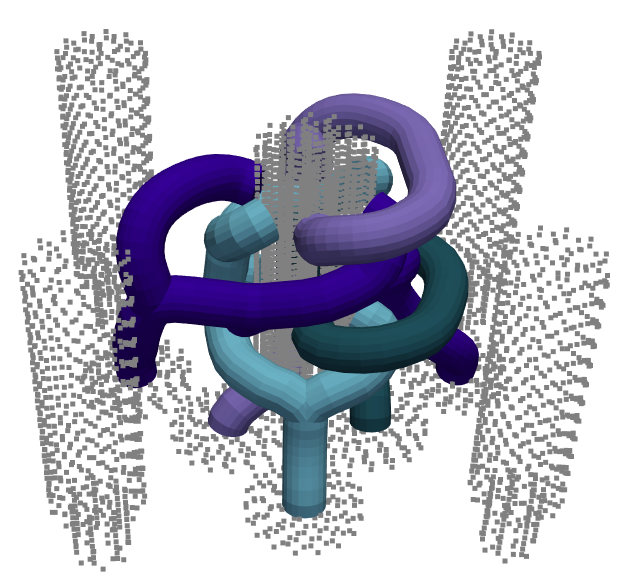
\includegraphics[width=0.72\linewidth]{figures/rotary_valve_pipes.png}
  \caption{Illustrative multi-group fluid channels around a center axis and
  structural pillars (visualisation of an AM-oriented valve-style layout).
  Coloured tubes are pipes of different groups; grey volumes mark occupied /
  forbidden structure. Channels are short and smoothly curved relative to
  drilled manifolds, but must not collide.}
  \label{fig:rotary-valve}
\end{figure}

AM makes such layouts manufacturable, but \emph{designing} the channels is
still a combinatorial 3D routing problem: many terminals, cluttered obstacles,
and hard clearance between groups. Manual CAD routing does not scale; we seek
automatic planners that return conflict-free multi-group layouts inside a
bounded design domain.

\section{From Valve Design to a Computational Problem}
\label{sec:problem}

We abstract the valve setting as \emph{multi-group pipe routing under permanent
geometric occupancy}. The design domain is a bounded 3D region with static
obstacles (housing, fasteners, sealed volumes, axis envelope, \ldots).
Terminals are partitioned into groups that may share a manifold toward the
axis; each routed pipe permanently occupies a tubular neighbourhood of radius
$r$ (there is no ``pass and release'' as in robot MAPF); cross-group geometric
interference is forbidden, while within-group sharing / branching is allowed
via a topology plan. This combination is not captured by classical MAPF
suites, so we formalize the problem below and construct a synthetic benchmark
(Sec.~\ref{sec:benchmark}).

\paragraph{Geometry and occupancy.}
The domain is discretised as a regular 3D grid of resolution $\Delta$
(we use $\Delta{=}1$ without loss of generality by scaling).
A pipe of radius $r$ occupies a \emph{capsule} neighbourhood along its
centreline (sphere swept along each segment). Static obstacles are modelled as
spheres, capsules, and/or axis-aligned boxes.
A query point (or cell centre) $p$ with pipe radius $r$ is \textbf{free} iff
its clearance to all static obstacles and to already committed pipes of
\emph{other} groups is at least $r$. Equivalently, the open ball $B(p,r)$ must
not intersect forbidden geometry.

\paragraph{Groups, terminals, and topology.}
An instance specifies $m$ groups $G_1,\ldots,G_m$. Group $G_i$ has terminals
$T_i=\{t_{i,1},\ldots,t_{i,n_i}\}$ on the domain boundary or on prescribed
interfaces such as the axis sleeve (ports in the valve metaphor; center-axis
openings may be additional terminals or topology goals).
Before geometric search, a topology builder maps $T_i$ to tasks (edges)
$E_i$---typically a spanning tree---and an optional intra-group growth order.
Solving all tasks of $G_i$ yields a connected tree-shaped network.
Cross-group tasks interact only through occupancy.

\paragraph{Conflicts.}
Unlike classical MAPF vertex/edge conflicts at a shared time, two pipes of
different groups conflict when their tubular neighbourhoods violate clearance.
A detected conflict stores witness points $(p_a,r_a)$ and $(p_b,r_b)$
(generally $p_a\neq p_b$) and a deficit measuring penetration.
Same-group contacts are not conflicts under the default sharing policy.

\paragraph{Feasible solution and objectives.}
A feasible solution is a set of paths for all tasks of all groups such that
every path is free w.r.t.\ static obstacles and all other-group committed
geometry.
The primary experimental objective in this paper is \emph{feasibility under a
wall-clock budget} (success rate). Secondary signals include total path cost
relative to a constructive witness.
Manufacturing-oriented criteria (bend count, supportability, pressure-loss
proxies) matter for valves but are left to future work; we focus on the
geometric multi-group core first.

\paragraph{Relation to MAPF.}
\begin{table}[htbp]
  \centering
  \caption{Classical MAPF vs.\ multi-group pipe routing under permanent
  occupancy.}
  \label{tab:vs-mapf}
  \begin{tabular}{@{}llp{0.36\linewidth}@{}}
    \toprule
    Aspect & Classical MAPF & This problem \\
    \midrule
    Occupancy & Temporary (agents move) & Permanent (pipes stay) \\
    Conflict & Same cell / edge @ time $t$ & Geometric clearance (dual witnesses) \\
    Agent & Single $s$--$t$ path & Multi-terminal \textbf{group} (tree) \\
    Time & Explicit time dimension & Design-time layout (no schedule) \\
    \bottomrule
  \end{tabular}
\end{table}
As shown in Table~\ref{tab:vs-mapf}, the settings differ in occupancy, conflict
semantics, and agent structure.
High-level MAPF controllers (CBS, PBS, priority planning) remain useful as
search over leaves (constraint sets or orders), provided low-level search and
conflict detection use permanent geometric occupancy.
We do not claim a drop-in replacement for spatiotemporal MAPF benchmarks.
